\documentclass[a4paper]{article}
\usepackage{graphicx}
\usepackage{array}
\usepackage{wrapfig,lipsum,booktabs}

\begin{document}
%name
\center{\textbf {\underline {\huge{Mukesh Prajapati}}}}




%address
\begin{flushleft}
{Flat no 01,\hfill{Contact : 9768879557} \\Plot no 59,60,\hfill{Email ID: mukeshprajapati0694@gmail.com}\\ Sector 5, \\Ghansoli.}
\end{flushleft}


\begin{figure}[h]
\begin{flushright}
\graphicspath{ {images/} }
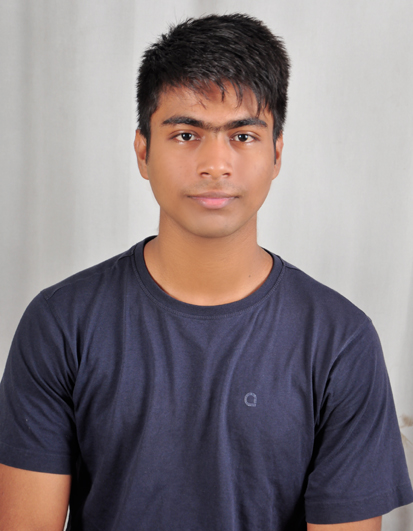
\includegraphics[width=3cm, height=4cm]{cv_pic}
\end{flushright}
\end{figure}

\begin{flushleft}
\textbf { EDUCATION}
\begin{center}
\begin{tabular}{ | m{2cm} | m{2.5cm}| m{2cm} | m{2.5cm}| m{3cm} | } 
\hline
Degree& College/School & University & Passing Year & Passing Percentage \\ 
\hline
10th  & St. Lawrence High School & Mumbai & 2011 & 60.36 \\ 
\hline
12th & Motilal Jhunjhun Wala Collage of Arta and Science & Mumbai & 2013 & 56.67 \\ 
\hline
B.E & Ramrao Adik Institute Of Technology & Mumbai & 2018 & 5.6 \\

\hline
\end{tabular}
\end{center}
\end{flushleft}


\begin{flushleft}
\textbf {PROJECTS}\\
\begin{itemize}
\item Level 1 wired robotics
\item level 2 wireless robotics
\item Smart water level controlling system using logic gates
\item Built a working model of an Elevator
\item Did a project called "Smart Suspention" for EYIC -2016 Symposium
\end{itemize}
\end{flushleft}

\begin{flushleft}
\textbf {TRAINING AND INTERNSHIP}\\
\begin{enumerate}
\item Attended work on "MORDEN DIGITAL DESIGIN" 
\item Was a faculty assistant for the workshop conducted on Arduino
\end{enumerate}
\end{flushleft}


\begin{flushleft}
\textbf \newline{RESEARCH PUBLICATION}
\begin{itemize}
\item Currently working for IEE-committee as a research wing member
\end{itemize}
\end{flushleft}
\end{document}

